\documentclass{article}

% if you need to pass options to natbib, use, e.g.:
% \PassOptionsToPackage{numbers, compress}{natbib}
% before loading nips_2017
%
% to avoid loading the natbib package, add option nonatbib:
% \usepackage[nonatbib]{nips_2017}

\usepackage[final,nonatbib]{nips_2017}

% to compile a camera-ready version, add the [final] option, e.g.:
% \usepackage[final]{nips_2017}

\usepackage[utf8]{inputenc} % allow utf-8 input
\usepackage[T1]{fontenc}    % use 8-bit T1 fonts
\usepackage{hyperref}       % hyperlinks
\usepackage{url}            % simple URL typesetting
\usepackage{booktabs}       % professional-quality tables
\usepackage{amsfonts}       % blackboard math symbols
\usepackage{nicefrac}       % compact symbols for 1/2, etc.
\usepackage{microtype}      % microtypography
\usepackage{graphicx}
\usepackage{amsmath}
\usepackage{wrapfig}
\usepackage{subcaption}
\usepackage[numbers]{natbib}
\usepackage[toc,page]{appendix}
\bibliographystyle{plainnat}
\begin{document}
\begin{appendices}

%-------------------------------------------------------------------------------
% Section A. Baseline Neuronal Boundary Detection
%-------------------------------------------------------------------------------
\section{Baseline Neuronal Boundary Detection}
\label{appendix:baseline}

In this section, we describe our baseline segmentation pipeline, which is
similar to what is described in~\cite{kisuk}. The major difference is our novel
densely multiscale 3D convolutional network architecture for neuronal boundary
detection, which will be described in detail in the following section. (The same
\emph{class} of architecture was employed in error detection and error
correction. See main text.)

\subsection{\textsl{DeltaNet}: a densely multiscale convolution network}
\label{sec:deltanet}

\begin{figure}[!b]
\centering
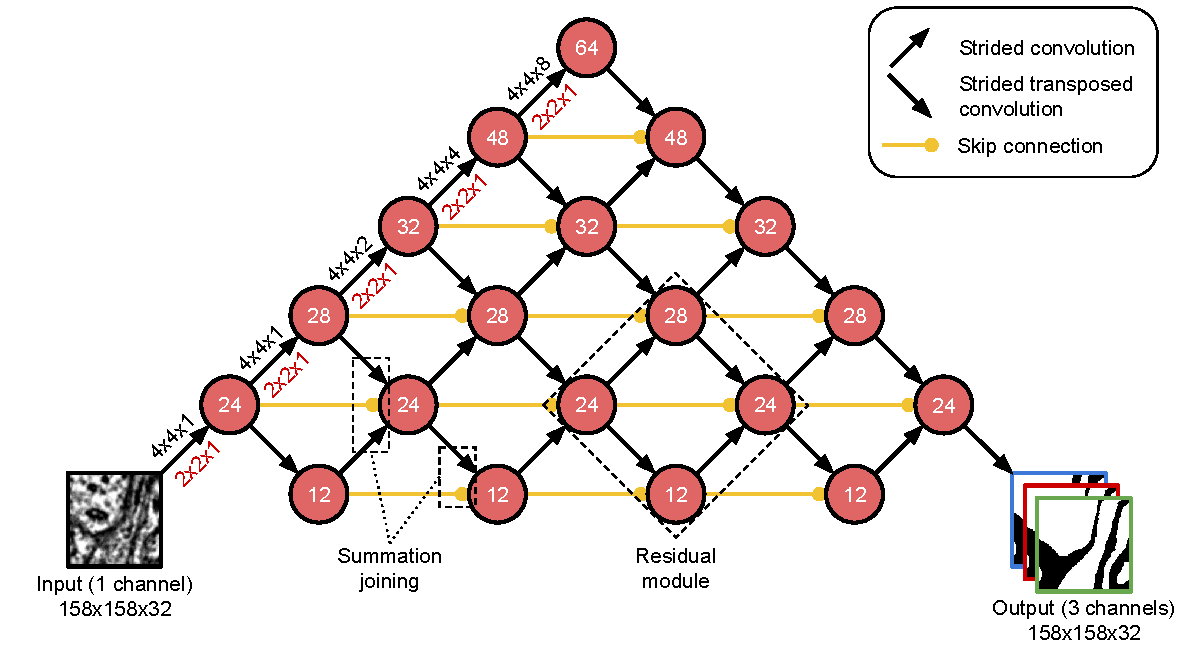
\includegraphics[width=1.0\linewidth]{baseline.pdf}

\caption{Architecture for the baseline neuronal boundary detection. Each node
represents a layer and the number inside represents the number of feature maps.
The layers closer to the top of the diagram have lower resolution than the
layers near the bottom. We make savings in computation by minimizing the number
of high resolution feature maps. The diagonal arrows represent strided
convolutions, while the horizontal arrows represent skip connections. Associated
with the diagonal arrows, black numbers indicate filter size and red numbers
indicate strides in $x\times y\times z$. The target for our boundary detection
net is a 3D \emph{affinity graph}~\cite{boundary_detection,kisuk,funke2017deep},
thus outputting three channels each corresponding to $x$ (green), $y$ (red), and
$z$ (blue) affinity map, respectively.}

\label{fig:boundary_detector}
\end{figure}

Our proposed densely multiscale 3D convolutional network (\emph{DeltaNet}) for
neuronal boundary detection is illustrated in
Figure~\ref{fig:boundary_detector}. DeltaNet is built upon U-Net~\cite{unet}
with several interesting architectural augmentation. DeltaNet can be viewed as a
pyramidal stack of the basic computational module (diamond-shaped box in
Figure~\ref{fig:boundary_detector}). This diamond-shaped module can be
interpreted as a residual building block (see Figure 2 in~\cite{resnet}) with
two residual pathways, one top-down and the other bottom-up. Thus DeltaNet is
\emph{fully residual} in the sense that every computational pathway involving
horizontal information flow is passing through the residual module. Moreover,
every residual module refines its input representation by integrating both
top-down and bottom-up information, thus allowing for \emph{dense} intermixing
of multiscale features. DeltaNet's \emph{dense} and \emph{fully residual}
architecture allows an incremental and iterative top-down/bottom-up refinement
of internal representation, which is in contrast to U-Net and variants' more
restricted coarse-to-fine top-down
refinement~\cite{pinheiro2016refine,lin2016pyramid}.

From a different point of view, Figure~\ref{fig:unfold} illustrates another
important motivation for our densely multiscale convolutional net architecture.
DeltaNet can be viewed as a feedback recurrent convolutional network unrolled in
time (Figure~\ref{fig:unfold}). Weight-sharing across time makes a DeltaNet
exactly equivalent to a convolutional net with recurrent feedback connections
unfolded through time, and this novel perspective provides a better framework
for understanding one of the unique characteristics of DeltaNet, i.e., the
incremental refinement of internal representation by interative integration of
top-down and bottom-up information. DeltaNet's internal representation is
incremetally and iteratively refined over time by integrating the top-down
contextual information conveyed through the feedback recurrent connnections and
the higer spatial-frequency information relayed through the bottom-up
feedforward connections.

\begin{figure}[!t]
\centering
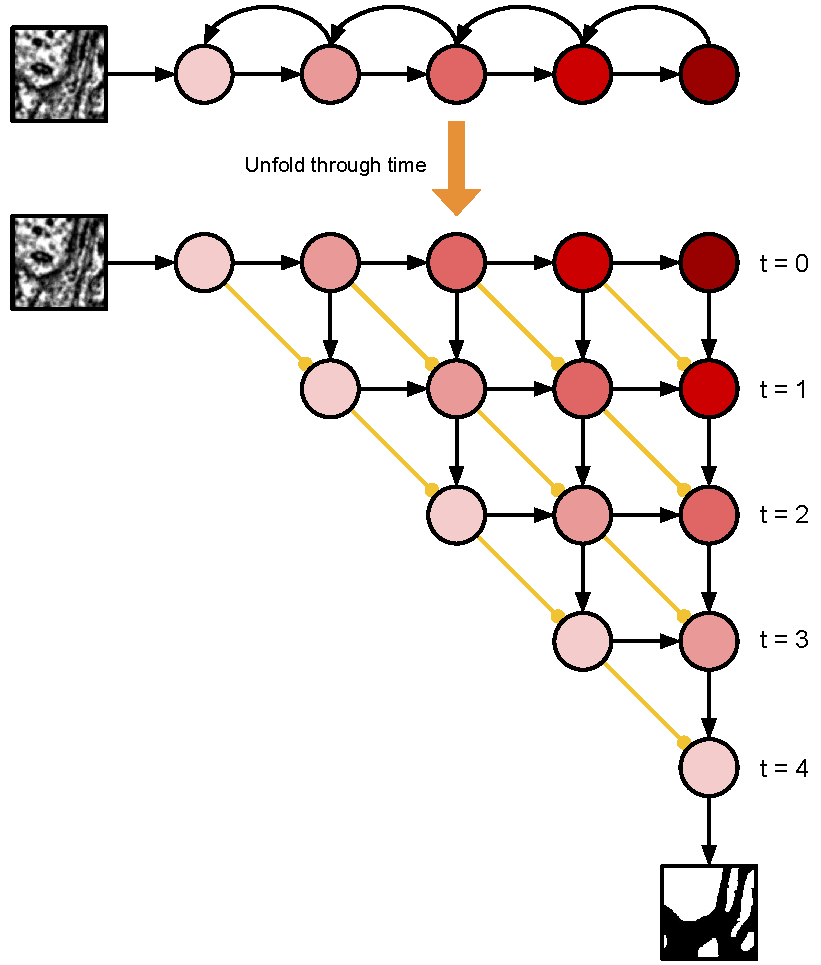
\includegraphics[width=0.65\linewidth]{unfold.pdf}

\caption{Feedback recurrent convolutional network unrolled in time.
See~\ref{sec:deltanet} for details}

\label{fig:unfold}
\end{figure}

\subsubsection{Architectural details} Due to the anisotropy of the resolution of
the images in our dataset, we design our nets so that the first convolutions are
exclusively 2D while later convolutions are 3D. The field of view of a unit in
the higher layers is therefore roughly cubic. To limit the number of parameters
in our model, we factorize all 3D convolutions into a 2D convolution followed by
a 1D convolution in $z$-dimension. We employed exponential linear units
(ELUs,~\cite{elu}) for nonlinearity, except for the output layer with logistic
activation functions.

\subsection{Dataset}
Our dataset is a sample of mouse primary visual cortex (V1) acquired using
transmission electron microscopy at the Allen Institute for Brain Science. The
voxel resolution is $3.6~\text{nm} \times 3.6~\text{nm} \times 40~\text{nm}$.

A team of tracers produced multiple volumes of gold standard dense reconstruction, in total $20$ volumes of size $512 \times 512 \times 100$. We trained our boundary detector using $19$ volumes and used the last volume for training validation. We then applied the trained boundary detector on a new image volume of size $2048 \times 2048 \times 100$ to obtain a preliminary segmentation, which was then proofread by the tracers to generate a bootstrapped ground truth volume. This volume was used to optimize the parameters for watershed and mean affinity agglomeration. Finally, the optimized segmentation pipeline was applied to generate further bootstrapped ground truth for the error detection and correction.

\subsection{Training procedures}
Our boundary detection networks were implemented based on the Caffe deep
learning framework~\cite{jia2014caffe}. To train our models, we minimized the
binomial cross-entropy loss with class-rebalancing using the Adam
optimizer~\cite{adam}, initialized with $\alpha=0.001$, $\beta_1=0.9$,
$\beta_2=0.999$, and $\epsilon=0.01$. The network weights were initialized
following He et al.~\cite{he2015delving}. The learning rate (or step size
parameter $\alpha$ in the Adam optimizer) was halved when validation loss
plateaued out, five times in total at $35$K, $175$K, $250$K, $300$K, and
$480$K training iterations. We used a single patch of size
$158\times158\times32$ (i.e. minibatch of size 1) to compute gradients at each
training iteration. The training lasted for $800$K iterations until convergence,
which took about five days on a single NVIDIA Titan X Pascal GPU.

\subsection{Inference and postprocessing}
We perform \emph{overlap-blending} inference followed by watershed and mean affinity agglomeration~\cite{kisuk}. We refer the interested readers to~\cite{kisuk} for further details.

%-------------------------------------------------------------------------------
% Section B. Network Architecture
%-------------------------------------------------------------------------------
\section{Per-object VI score}
\label{appendix:vi}
 Recall that the variation of information between two segmentations may be computed as
\begin{align*}
	VI_\text{split}&=-\frac 1 {\sum_{i,j} r_{ij}} \sum_{i,j} r_{ij} \log(r_{ij}/p_i),\\
	VI_\text{merge}&=-\frac 1 {\sum_{i,j} r_{ij}} \sum_{i,j} r_{ij} \log(r_{ij}/q_j),\\
	p_i&=\sum_j r_{ij},\\
	q_j&=\sum_i r_{ij},
\end{align*}
where $r_{ij}$ is the number of voxels in common between the $i^\text{th}$ segment of the ground truth segmentation and the $j^\text{th}$ segment of the proposed segmentation \cite{vi}.

We define the split and merge scores for ground truth segment $i$ as
\begin{align*}
	VI_\text{split}(i) &= -\sum_j r_{ij}/p_i \log(r_{ij}/p_i),\\
	VI_\text{merge}(i) &= -\sum_j r_{ij}/p_i \log(r_{ij}/q_j),
\end{align*}
Both quantities have units of bits. $VI_\text{split}(i)$ is zero iff ground truth segment $i$ is contained within a segment in the proposed segmentation, while $VI_\text{merge}(i)$ is zero iff ground truth segment $i$ is the union of one or more segments in the proposed segmentation. The total score $VI_\text{split}$ or $VI_\text{merge}$ is a weighted sum of the per-object scores $VI_\text{split}(i)$, $VI_\text{merge}(i)$ respectively.


%-------------------------------------------------------------------------------
% Section B. Training Details
%-------------------------------------------------------------------------------
\section{Training details}
The neural networks were implemented in TensorFlow \cite{tensorflow} and trained
using 4 TitanX Pascal GPUs with synchronous gradient descent. We used the Adam
optimizer \cite{adam}, initialized with $\alpha=0.001$, $\beta_1=0.95$,
$\beta_2=0.9995$, and $\epsilon=0.1$. Both networks were trained until the loss
on a validation set plateaued. The error detection network trained for $700$K
iterations (approximately one week), while the error-correcting network trained
for $1.7$M iterations (approximately three weeks).

\end{appendices}

\bibliography{bib}

\end{document}
